% Results figures, rendered from the persisted artifacts:
% bootstrap_ci.json (suite means and 95% CIs), stability_run1_vs_run2.json (run pairs).
% Values resolve through figures/generated_values.tex, which scripts/gen_sp_figures.py
% writes from those artifacts; run `python scripts/gen_sp_figures.py --check` to prove
% this figure still agrees with them.
% Layout discipline: the top panel shows point estimates + intervals only
% (no filled bars under the whiskers), the bottom panel's legend lives
% below the axis (never over the bars), and both panels share the same
% value range so the stacked scales read as one.
% GENERATED by scripts/gen_sp_figures.py -- do not edit by hand.
% Every plotted number in the S&P figures resolves through this file, so a
% figure cannot silently disagree with the artifact it claims to show.
% Regenerate:  python scripts/gen_sp_figures.py
% Verify:      python scripts/gen_sp_figures.py --check
% Sources:
%   results/bootstrap_ci.json
%   results/stability_run1_vs_run2.json
%   results/b4_baseline_zodiac_20260922.json
%   results/model_quality/chrollo_calibration.json
%   results/sp2027_rescue/behavior_trajectory_benchmark.json

\def\RaginLiveTechnique{0.9598}
\def\RaginLiveTechniqueErrLo{0.0122}
\def\RaginLiveTechniqueErrHi{0.0122}
\def\RaginLiveActor{0.8500}
\def\RaginLiveActorErrLo{0.0000}
\def\RaginLiveActorErrHi{0.0000}
\def\RaginLivePersona{0.7325}
\def\RaginLivePersonaErrLo{0.0587}
\def\RaginLivePersonaErrHi{0.0558}
\def\RaginLiveComposite{0.8796}
\def\RaginLiveCompositeErrLo{0.0224}
\def\RaginLiveCompositeErrHi{0.0204}
\def\RaginLivePersonaRunTwo{0.7504}
\def\RaginLiveCompositeRunTwo{0.8845}
\def\RaginPersonaRunDelta{0.018}
\def\RaginTechDelta{0.317}
\def\RaginTechDeltaLo{0.162}
\def\RaginTechDeltaHi{0.480}
\def\RaginActorDelta{0.140}
\def\RaginActorDeltaLo{0.083}
\def\RaginActorDeltaHi{0.197}
\def\RaginPersonaNullDelta{0.005}
\def\RaginPersonaNullDeltaLo{-0.047}
\def\RaginPersonaNullDeltaHi{0.057}
\def\RaginOverallDelta{0.154}
\def\RaginOverallDeltaLo{0.092}
\def\RaginOverallDeltaHi{0.221}
\def\RaginGroundingTtpCount{35}
\def\RaginNoGroundingTtpCount{0}
\def\RaginRoutingBefore{0.8875}
\def\RaginRoutingAfter{0.955}

\begin{figure}[t]
\centering
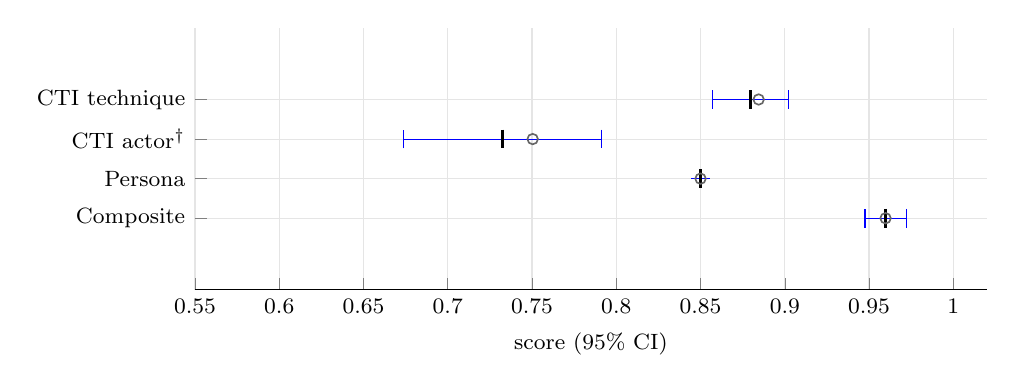
\begin{tikzpicture}
\begin{axis}[
  name=ax1,
  width=0.96\linewidth,
  height=4.9cm,
  xmin=0.55, xmax=1.02,
  y axis line style={draw=none},
  axis x line*=bottom,
  axis y line*=left,
  ytick=data,
  yticklabels={Composite,Persona,CTI actor$^{\dagger}$,CTI technique},
  y dir=reverse,
  xlabel={score (95\% CI)},
  xlabel style={font=\footnotesize},
  tick label style={font=\footnotesize},
  enlarge y limits=0.6,
  grid=major,
  grid style={black!10},
  clip=false
]
% point estimates and bootstrap 95% CIs from bootstrap_ci.json;
% only marks + intervals: no bars beneath the whiskers
\addplot+[only marks, mark=|, mark size=3.4, mark options={thick,black},
  error bars/.cd, x dir=both, x explicit] coordinates {
  (\RaginLiveTechnique,3) +- (\RaginLiveTechniqueErrLo,\RaginLiveTechniqueErrHi)
  (\RaginLiveActor,2) +- (\RaginLiveActorErrLo,\RaginLiveActorErrHi)
  (\RaginLivePersona,1) +- (\RaginLivePersonaErrLo,\RaginLivePersonaErrHi)
  (\RaginLiveComposite,0) +- (\RaginLiveCompositeErrLo,\RaginLiveCompositeErrHi)
};
% run-2 overlay: open markers (point estimates from stability_run1_vs_run2.json;
% per-suite CIs were not computed for run 2, so none are drawn)
\addplot+[only marks, mark=o, mark size=1.9, mark options={semithick,black!60}] coordinates {
  (\RaginLiveTechnique,3)
  (\RaginLiveActor,2)
  (\RaginLivePersonaRunTwo,1)
  (\RaginLiveCompositeRunTwo,0)
};
\end{axis}
\end{tikzpicture}

\vspace{2mm}

\begin{tikzpicture}
\begin{axis}[
  name=ax2,
  width=0.96\linewidth,
  height=4.9cm,
  ybar=1.5pt,
  bar width=9pt,
  ymin=0.55, ymax=1.0,
  symbolic x coords={CTI technique,CTI actor,Persona,Composite},
  xtick=data,
  ylabel={mean score},
  ylabel style={font=\footnotesize},
  tick label style={font=\footnotesize},
  ymajorgrids,
  grid style={black!10},
  enlarge x limits=0.25,
  legend style={font=\scriptsize, at={(0.5,-0.16)}, anchor=north, legend columns=2, draw=none, fill=none},
  legend cell align={left},
]
% run 1 vs run 2 from stability_run1_vs_run2.json
\addplot+[black!35, fill=black!35] coordinates {
  (CTI technique,\RaginLiveTechnique) (CTI actor,\RaginLiveActor) (Persona,\RaginLivePersona) (Composite,\RaginLiveComposite)
};
\addplot+[black!70, fill=black!70, pattern=north east lines] coordinates {
  (CTI technique,\RaginLiveTechnique) (CTI actor,\RaginLiveActor) (Persona,\RaginLivePersonaRunTwo) (Composite,\RaginLiveCompositeRunTwo)
};
\legend{run 1, run 2}
\end{axis}
\end{tikzpicture}
\caption{Live-campaign results from the persisted artifacts (identical
deterministic-strata bars across runs are the finding, not a plotting
error). All four plotted values are the \emph{both-channel} operational
score of Table~\ref{tab:live}, which fuses the served-text and CTI-analysis
channels; they are not served-quality results, and the echo-guarded bounds
for the same rows are 0.479 technique and 0.243 actor.
\emph{Top:}
suite means with bootstrap 95\% confidence intervals; open markers mark
the independent second run's point estimates, and the actor interval is
degenerate ($^{\dagger}$) because the actor rubric assigns the same
score to every row, so uncertainty is carried by the Wilson pass-rate
interval instead (Table~\ref{tab:live}). \emph{Bottom:} two independent
218-query campaigns; the deterministic CTI strata replicate exactly and
only the LLM-judged persona stratum moves, by $+\RaginPersonaRunDelta$.}
\label{fig:results}
\end{figure}
